\documentclass[sigconf,nonacm]{acmart}

\settopmatter{printacmref=false}
\setcopyright{none}
\renewcommand\footnotetextcopyrightpermission[1]{}
\acmConference[Security Insider Lab II]{Security Insider Lab II Mini Project}{July 2026}{University of Passau}
\acmYear{2026}
\copyrightyear{2026}

\usepackage{booktabs}
\usepackage{array}
\usepackage{tikz}
\usetikzlibrary{arrows.meta,positioning}

\begin{document}

\title{HermSec: A User-Friendly Repository Security Scanner with a Comparison of Static, Single-Agent, Multi-Agent, and Hybrid Review Modes}

\author{Seth Whenton}
\affiliation{%
  \institution{University of Passau}
  \city{Passau}
  \country{Germany}}
\email{}

\begin{abstract}
HermSec is a desktop security scanner for local repositories. It is built to help a developer choose a project, inspect what kind of code it contains, prepare the right scanner tools, run the scan, and generate a readable report. The app includes a chat workflow, live progress cards, scanner settings, model provider settings, doctor checks, automations, and HTML/PDF/JSON reports.

This paper first presents HermSec as a product, then compares four review modes. Deep assisted scan runs static scanners and uses a model to explain scanner evidence. Single agent inspection lets one model inspect bounded code snippets without scanners. MoA inspection uses several specialist agents, a false-positive judge, and an aggregator without scanners. Scanner + MoA inspection runs scanners and MoA together, then uses a judge and final aggregator to validate both sets of findings.

A broad earlier scanner-only test found 89 of 184 planted vulnerabilities across 11 languages. The final comparison used four smaller fixtures with 12 planted vulnerabilities. Deep assisted scan had the best recall at 0.667, but low precision at 0.090 because it produced many extra findings. Single agent inspection had precision 0.667, but recall 0.167. MoA inspection reached F1 0.476. Scanner + MoA reached the best F1 score at 0.500. The result suggests that HermSec works best when broad scanner coverage is combined with agent-based filtering.
\end{abstract}

\keywords{static analysis, software security, large language models, multi-agent systems, vulnerability detection, code review}

\maketitle

\section{Introduction}
Developers need security feedback while they write code. Static application security testing tools can help because they scan source code without running the program \cite{chess2004static,livshits2005finding}. These tools are useful, but they also have limits. They need good rules, language support, and careful tuning. If the rules are weak, the tool can miss real bugs. If the rules are too broad, the tool can report too many false alarms \cite{zitser2004testing}.

HermSec is a desktop app that scans projects for security issues. It uses built-in rules and external tools such as Semgrep, Gitleaks, Trivy, Bandit, and other scanners \cite{semgrep,gitleaks,trivy,bandit}. The app also supports model-assisted review. During testing, one clear problem appeared. Scanner-based reports found many issues, but they could become noisy. Model-only review was easier to read, but it missed more issues.

The main product idea is simple. A user should be able to pick a repository and ask HermSec to scan it. HermSec then inspects the project, checks the language and project files, chooses the scanner tools that fit that project, prepares or installs missing managed tools, runs the scan, and writes a report. This is important because a React project, Java project, Python project, and Rust project should not all need the same scanner setup.

This project studies a simple question: can agent review improve HermSec's scanner reports without losing too much coverage?

The paper compares four HermSec modes:

\begin{itemize}
  \item \textbf{Deep assisted scan}: HermSec runs scanners first. The model then explains scanner evidence when possible.
  \item \textbf{Single agent inspection}: One model reads selected code evidence and writes findings. No scanners run in this mode.
  \item \textbf{MoA inspection}: Several specialist agents inspect the code. A judge checks possible false positives. An aggregator writes the final report.
  \item \textbf{Scanner + MoA inspection}: HermSec runs scanners and MoA review, then a judge and final aggregator validate both sets of findings.
\end{itemize}

This paper does not claim that agents are always better than scanners. The goal is smaller and clearer. It tests how the four modes behave on controlled examples and explains what should be improved next.

Figures~\ref{fig:hermsec-workflow} and~\ref{fig:hermsec-settings} show parts of the HermSec app that were built during the project. The scan workflow asks the user to choose a mode, shows live progress, and then writes a short result summary. The settings screens let the user configure agent modes and model providers.

\begin{figure*}
  \centering
  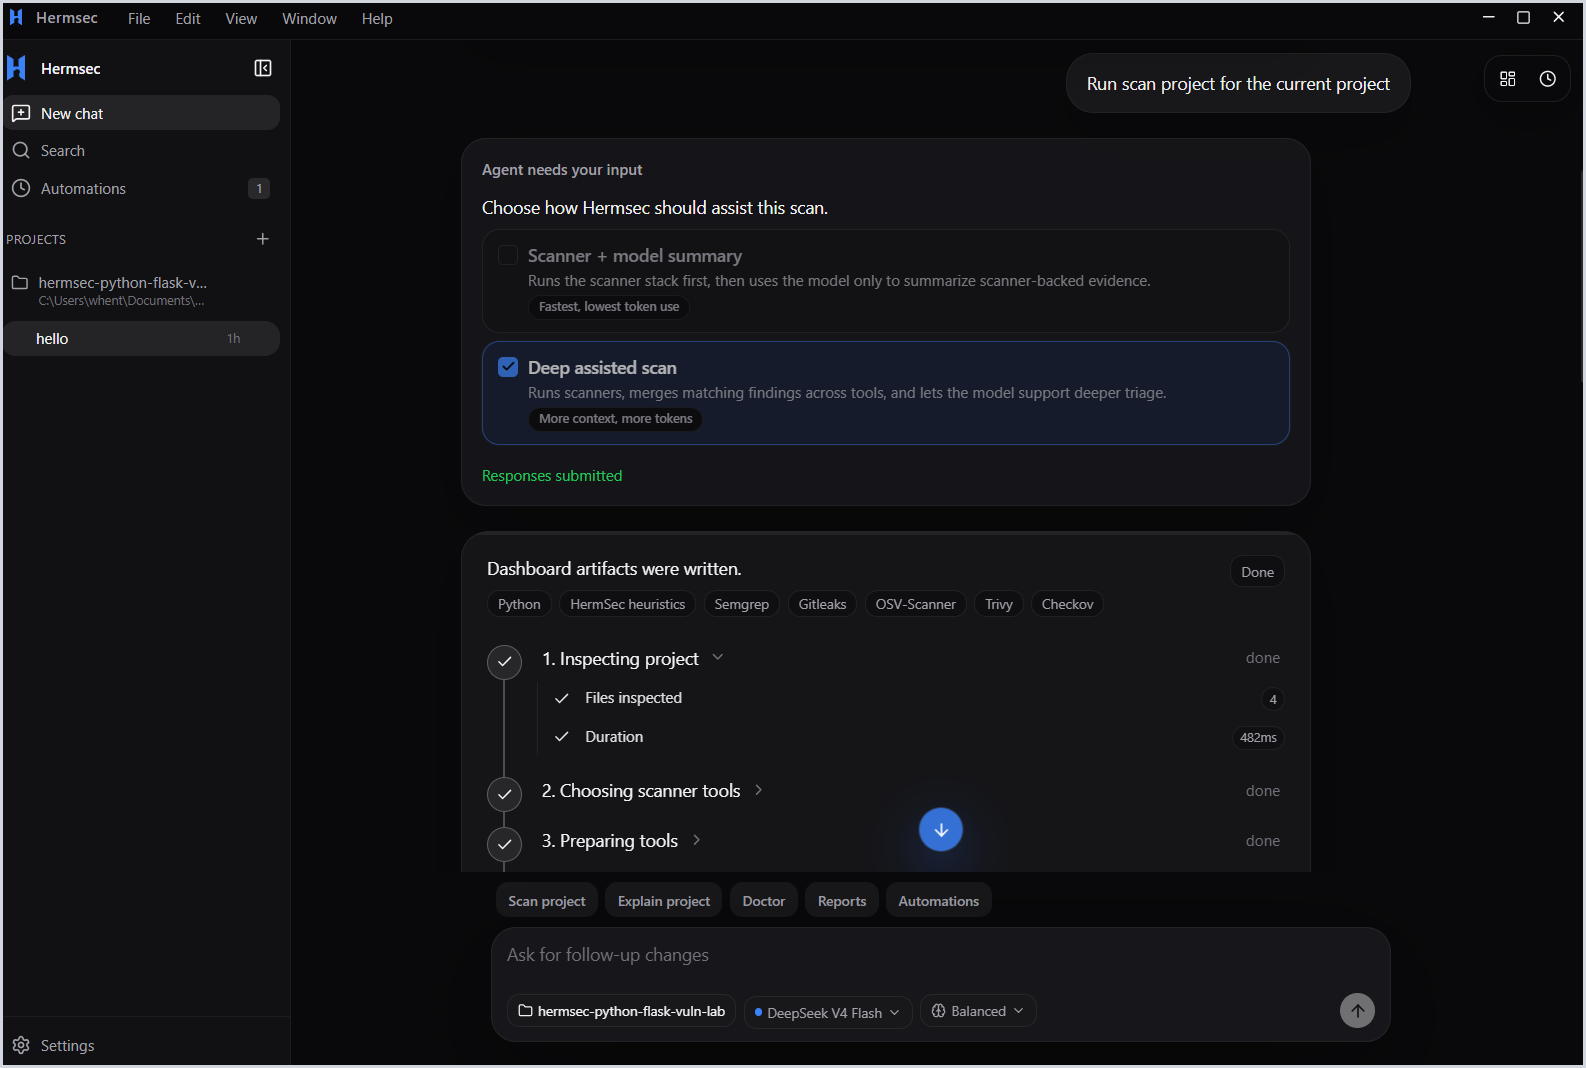
\includegraphics[width=.49\textwidth]{figures/hermsec_scan_choice_progress.png}\hfill
  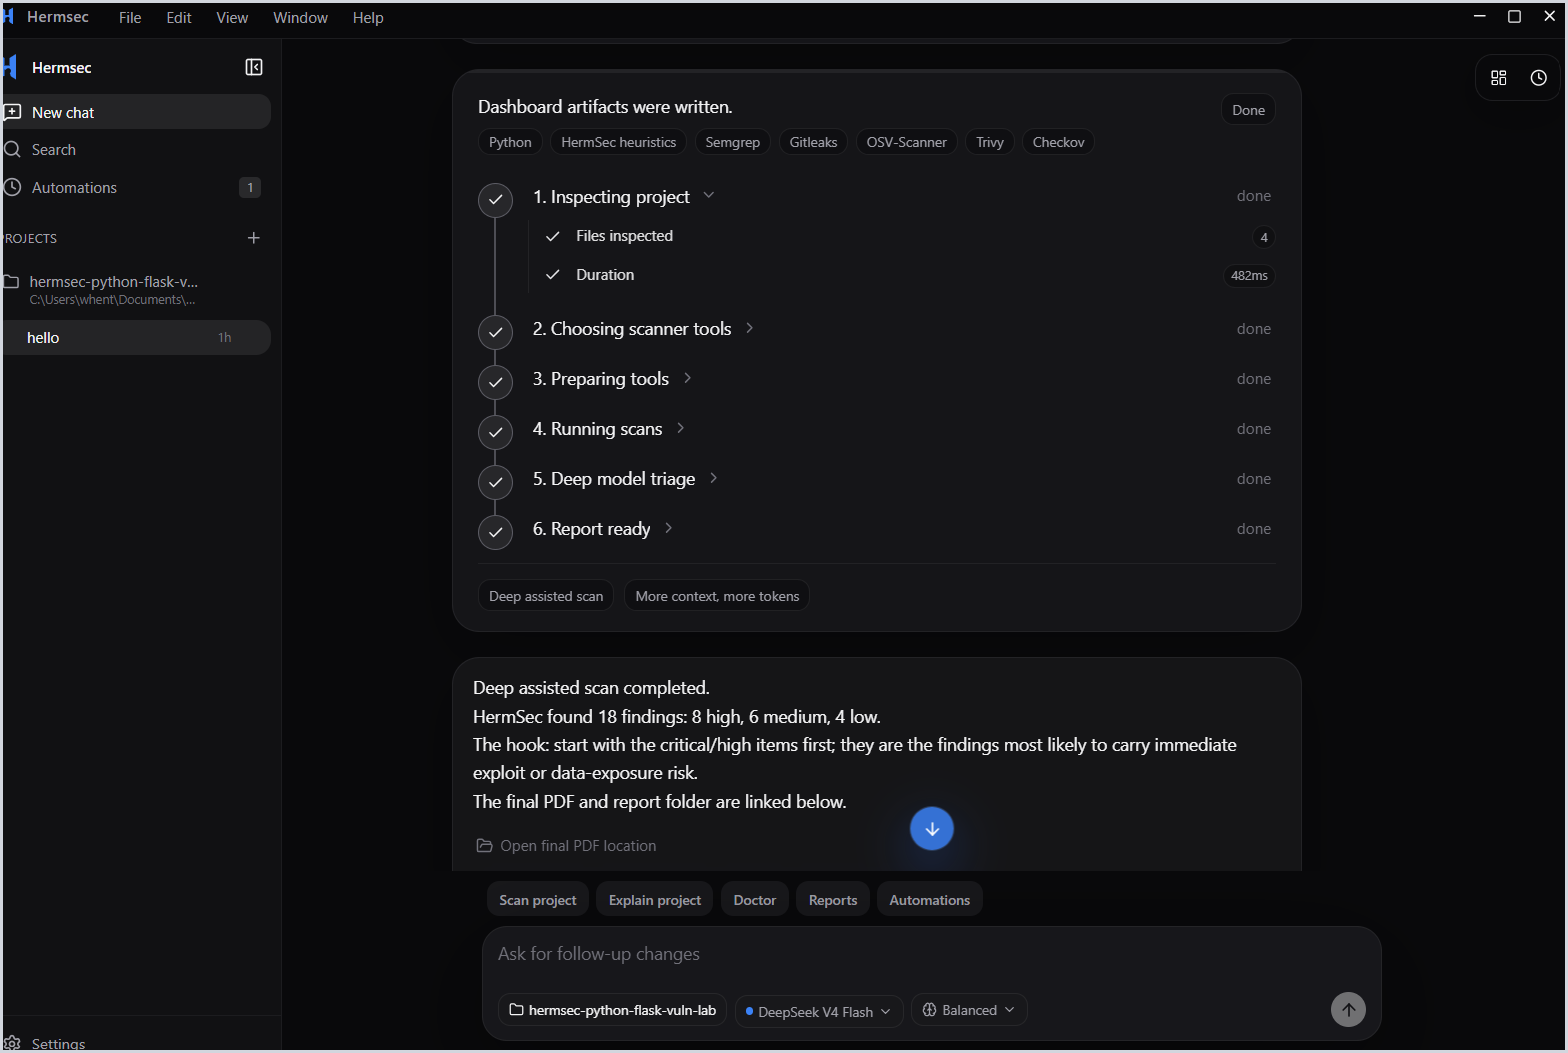
\includegraphics[width=.49\textwidth]{figures/hermsec_scan_completed_summary.png}
  \caption{HermSec scan workflow. Left: the user chooses a scan mode and sees live progress. Right: the scan finishes and HermSec shows a short summary with report links.}
  \Description{Two screenshots of the HermSec desktop application. The left screenshot shows scan mode selection and a live progress card. The right screenshot shows the completed progress card and the final chat summary.}
  \label{fig:hermsec-workflow}
\end{figure*}

\begin{figure*}
  \centering
  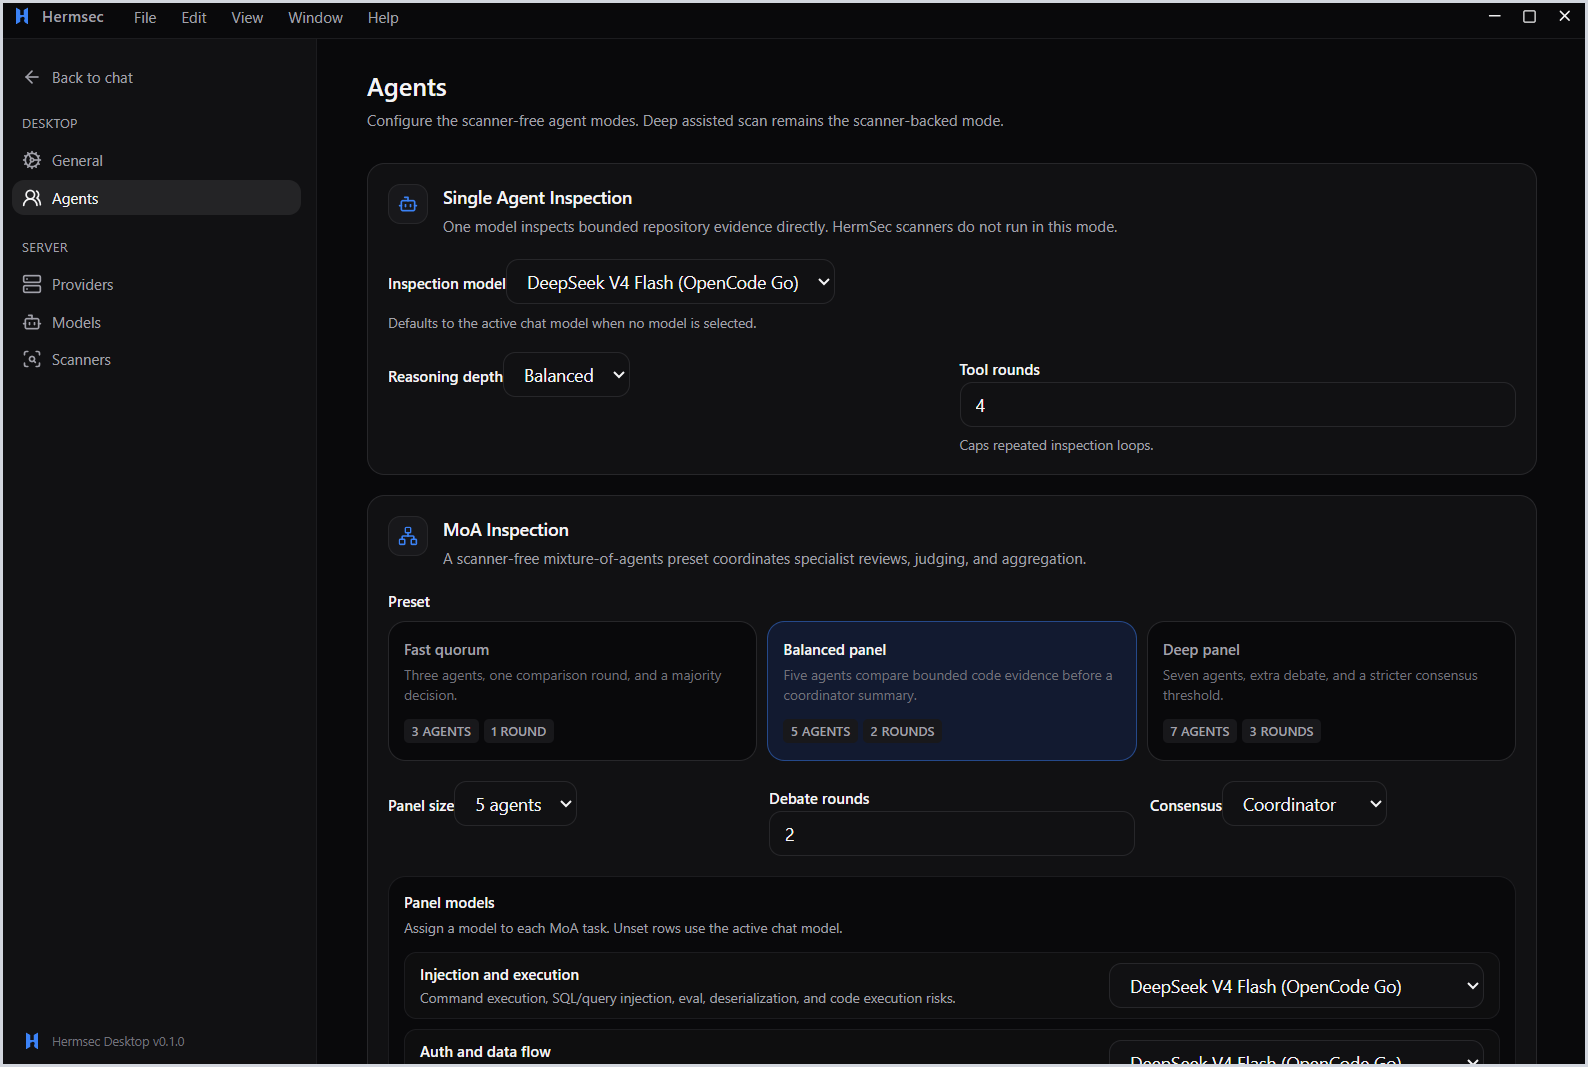
\includegraphics[width=.49\textwidth]{figures/hermsec_agents_settings_full.png}\hfill
  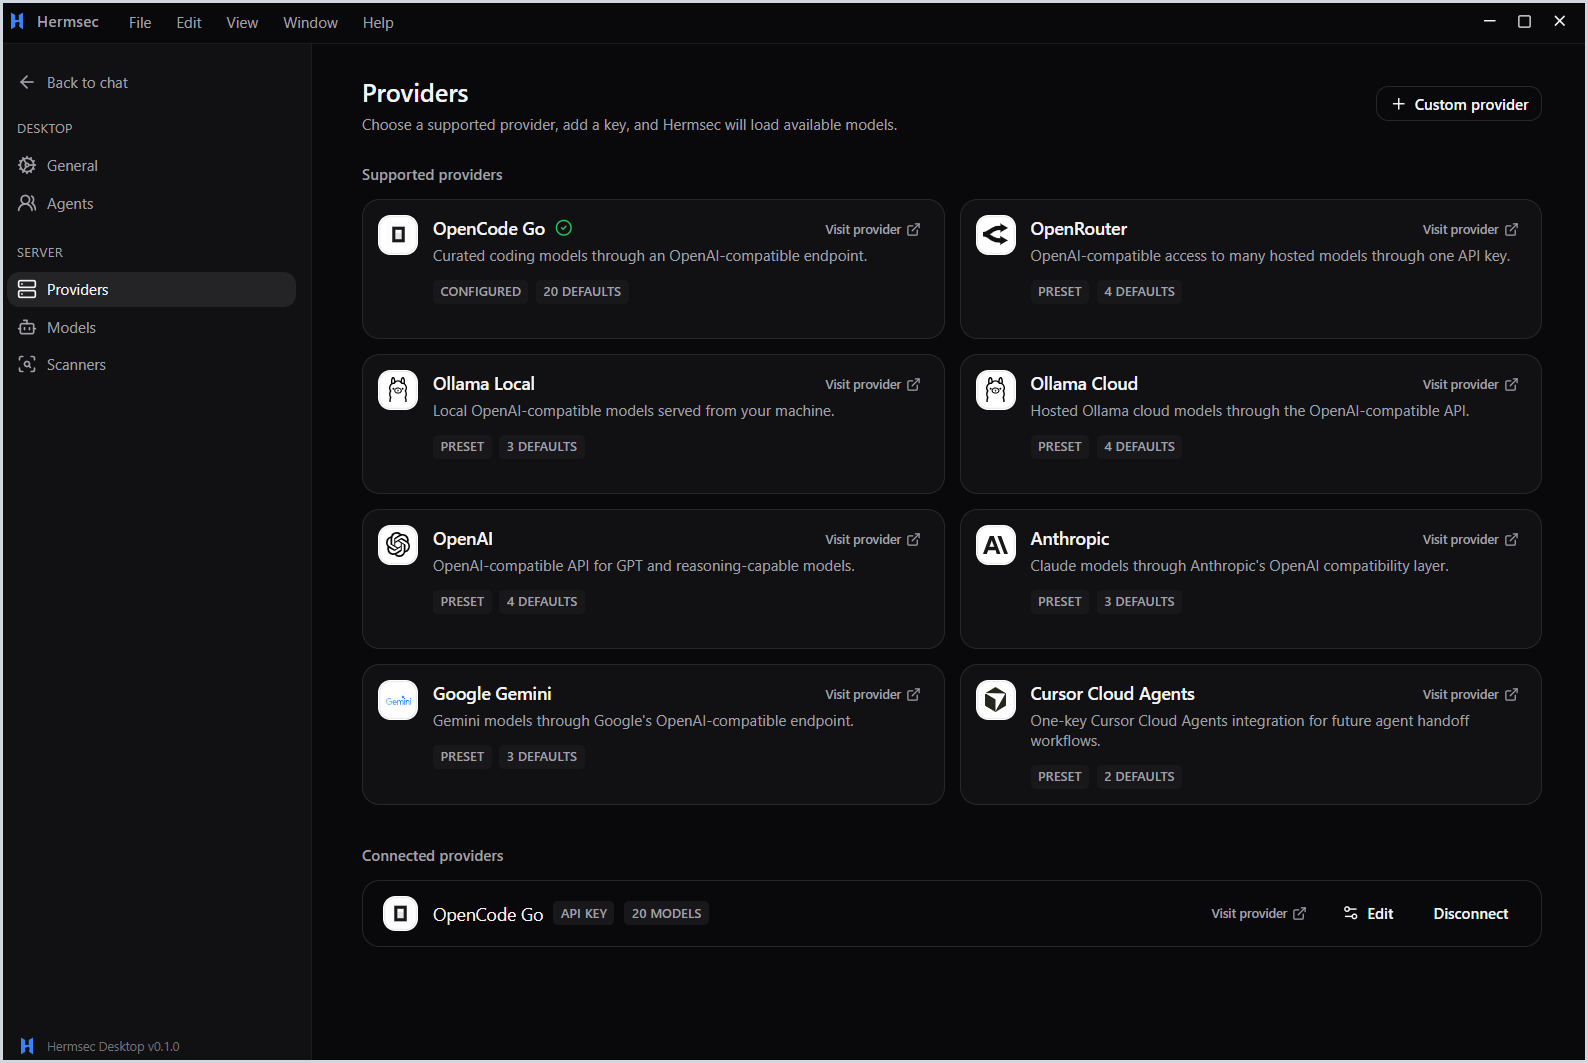
\includegraphics[width=.49\textwidth]{figures/hermsec_providers_settings.png}
  \caption{HermSec settings screens. Left: Agents settings for Single Agent and MoA inspection. Right: provider setup with OpenCode Go and other supported providers.}
  \Description{Two screenshots of the HermSec settings screens. The left screenshot shows Single Agent and MoA settings. The right screenshot shows provider cards and a connected OpenCode Go provider.}
  \label{fig:hermsec-settings}
\end{figure*}

\section{HermSec Product Overview}
HermSec is not only a benchmark script. It is a desktop application for normal developers who want a simple way to check a local project. The main screen is a chat interface. The user selects a project folder, chooses a scan mode, and watches the scan progress in the chat. When the scan ends, HermSec writes report files and gives links to the report folder and PDF.

HermSec also has a project inspection step. Before running a scan, it checks the repository files, languages, manifests, lockfiles, and configuration files. From this profile, HermSec chooses the scanners that make sense for the project. For example, a Node.js project can use JavaScript rules, npm audit style checks, secret scanning, OSV, and Trivy. A Python project can use Python rules, Bandit, pip-audit, OSV, and Trivy. This keeps the scan workflow smaller and avoids installing every possible tool for every project.

The scanner manager is part of the product. It shows which scanners are installed, missing, enabled, and used by the current project. Supported scanners can be installed into HermSec's managed tool directory instead of being forced into the user's global system path. Figure~\ref{fig:hermsec-scanners} shows this scanner settings screen.

Other product features include Doctor checks, model provider setup, model selection, agent settings, scan automations, live progress cards, and HTML/PDF/JSON reports. The Doctor checks confirm that scanner tools, internet connectivity, and provider setup are ready. The report system keeps the final result readable instead of only printing raw scanner output.

\begin{figure}
  \centering
  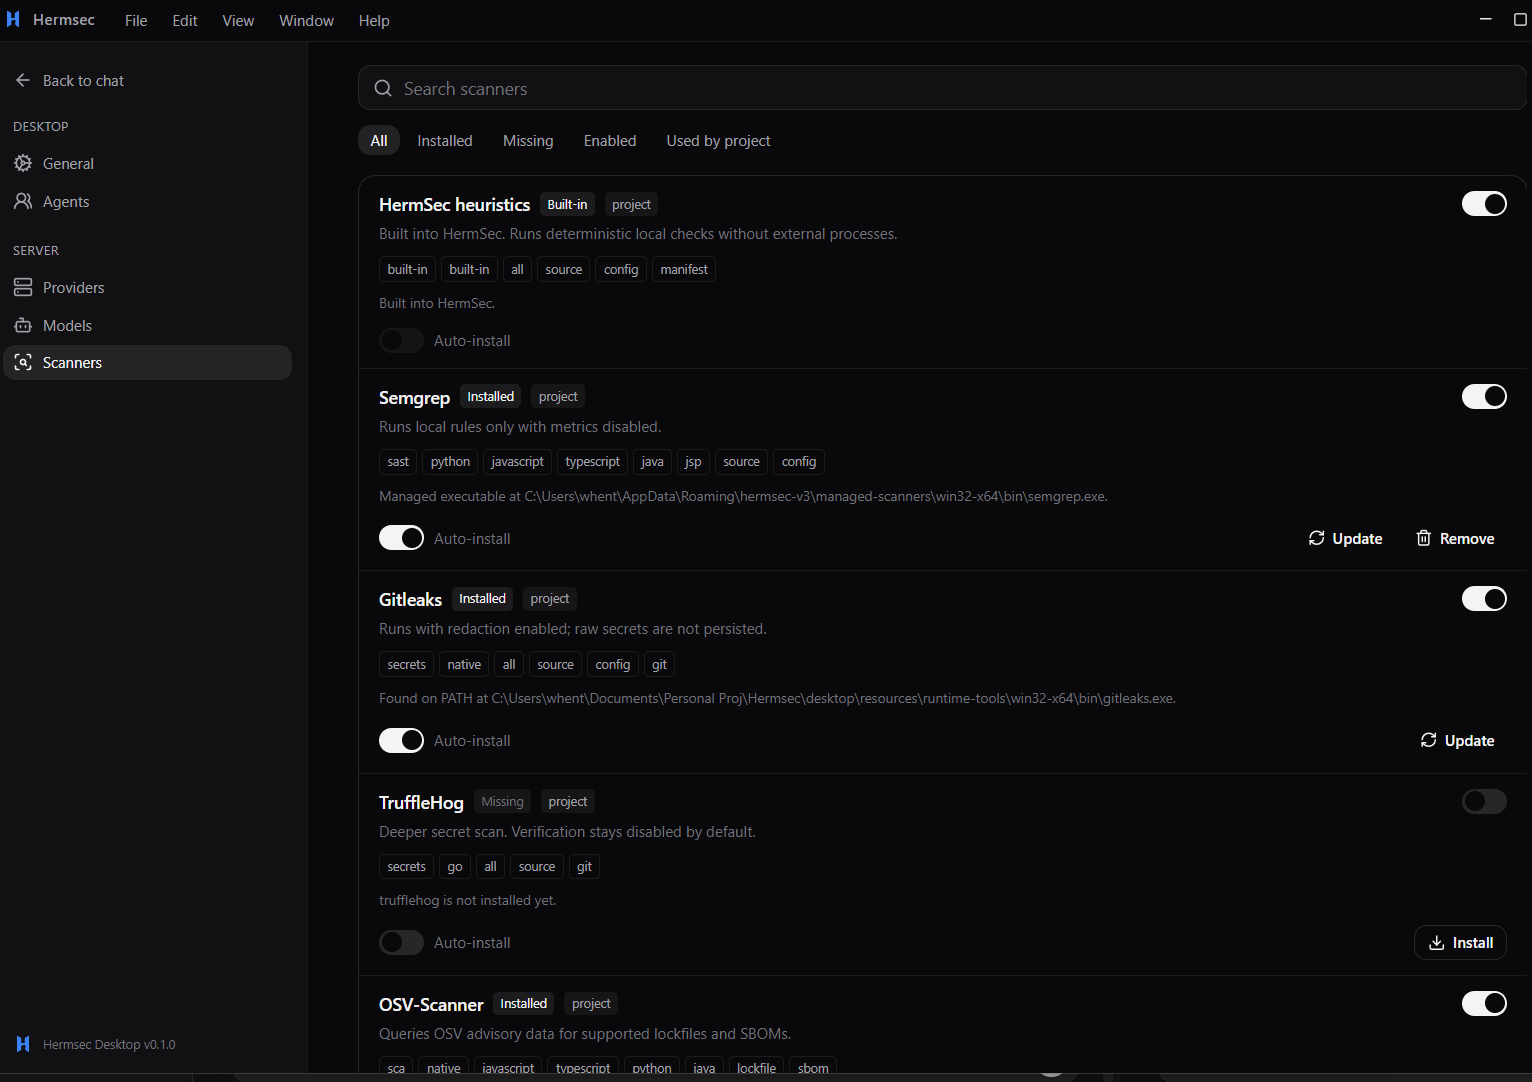
\includegraphics[width=\linewidth]{figures/hermsec_scanners_settings.png}
  \caption{HermSec scanner settings. The app shows installed, missing, enabled, and project-relevant scanners.}
  \Description{A screenshot of the HermSec scanners settings page showing scanner rows for HermSec heuristics, Semgrep, Gitleaks, TruffleHog, and OSV-Scanner.}
  \label{fig:hermsec-scanners}
\end{figure}

\section{Background and Related Work}
\subsection{Static Security Analysis}
Static analysis checks code before the program runs. It is often used to find security problems such as injection, unsafe data flow, and dangerous API use \cite{chess2004static,livshits2005finding}. However, static tools must be tested with known examples. A tool may look strong in one project and weak in another project \cite{zitser2004testing}.

Security benchmarks help make this testing fair. OWASP Benchmark and NIST Juliet are examples of test suites with known bugs \cite{owaspbenchmark,nistjuliet}. This project uses the same idea, but with smaller local fixtures. The findings are labelled with CWE identifiers from MITRE CWE \cite{mitrecwe}. The tested vulnerability types also match common web security risks, such as injection, cross-site scripting, weak cryptography, hardcoded secrets, and unsafe configuration \cite{owasptop10}.

\subsection{Scanner Harnesses}
Many security tools combine several scanners. This is because one scanner usually does not cover every language or every type of vulnerability. HermSec follows this approach. Semgrep gives general static analysis coverage. Gitleaks finds secrets. Trivy finds dependency, secret, and configuration issues. Bandit improves Python coverage \cite{semgrep,gitleaks,trivy,bandit}.

This scanner approach is fast and useful. The main problem is that scanner outputs must be cleaned and merged. If HermSec only lists every scanner result, the user may see duplicates or low-value findings. For this reason, HermSec normalizes findings and stores evidence for each issue.

\subsection{LLM Agents and MoA}
Large language models can read code and explain risks, but they can also make mistakes \cite{pearce2022asleep}. Agent systems try to make model work more controlled by giving the model tools and steps. ReAct is one example of combining reasoning with actions such as searching or reading files \cite{yao2023react}.

Multi-agent work also shows that several model responses can sometimes improve the final answer \cite{du2023debate,wang2024moa}. HermSec's MoA mode uses this idea for code security review. Different agents focus on different risk areas. Then a judge removes weak findings, and an aggregator writes the final report. This idea was also inspired by the configurable agent panels in Hermes Agent \cite{nous2026hermesagent}.

\section{System Design}
\subsection{Deep Assisted Scan}
Deep assisted scan is the scanner-based mode. HermSec first inspects the project. It chooses scanner tools, prepares them, runs them, and normalizes the findings. After that, the model can explain the scanner-backed evidence. If the model step fails, HermSec can still write a report from scanner findings. This is the closest mode to the original HermSec idea: a simple repository scanner that selects the right security tools for the project.

\subsection{Single Agent Inspection}
Single agent inspection does not run scanners. One model inspects the repository using safe read-only tools. It can list files, search code, and read snippets. It must report the file path, line or snippet, vulnerability category, evidence, confidence, and remediation. HermSec checks the evidence before adding the finding to the report.

\subsection{MoA Inspection}
MoA means mixture of agents. In this mode, HermSec runs a panel of specialist agents. The default roles include injection, secrets and supply chain, authentication, crypto and data protection, configuration and IaC, language and framework, API security, and database security. A false-positive judge checks the candidates. The aggregator then writes the final accepted findings.

\subsection{Scanner + MoA Inspection}
Scanner + MoA inspection is the hybrid mode added after the first tests. In this mode, scanners run and produce candidate findings. MoA agents also inspect the repository with bounded read-only code tools. Then a false-positive judge reviews both scanner findings and agent findings together. Finally, an aggregator writes the accepted and deduplicated findings into the normal HermSec report. The goal is to keep the broad coverage of scanners while using agents to reduce false positives and improve the final explanation.

\subsection{Safety Limits}
The agent modes are limited on purpose. They cannot run shell commands. They cannot install packages. They cannot execute project scripts. They cannot read outside the selected repository. HermSec also skips noisy folders such as \texttt{.git}, \texttt{node\_modules}, build folders, and vendored code. These limits make the agent modes safer and easier to test.

\begin{figure*}
  \centering
  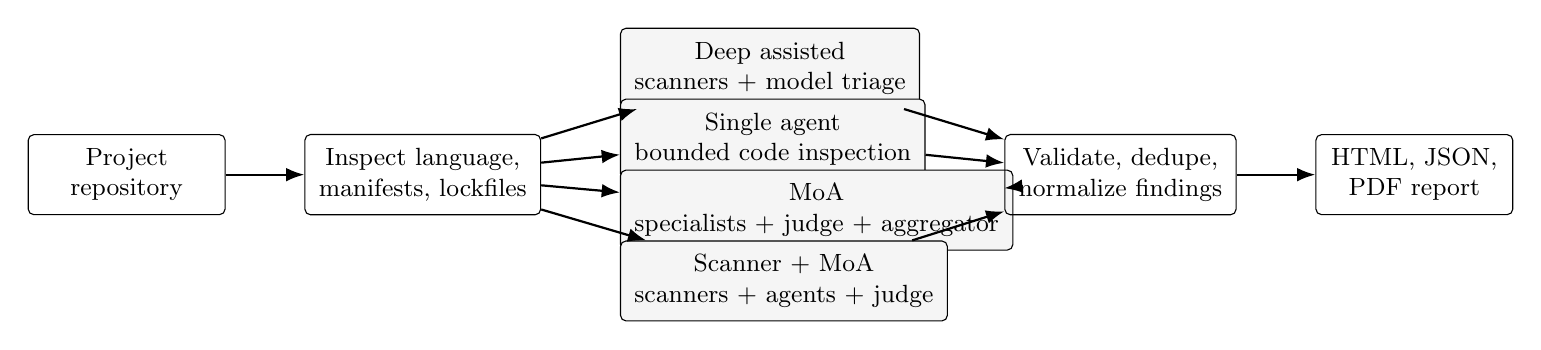
\begin{tikzpicture}[
    font=\small,
    box/.style={draw, rounded corners=2pt, align=center, inner sep=5pt, minimum width=2.5cm, minimum height=.72cm},
    mode/.style={draw, rounded corners=2pt, align=center, inner sep=5pt, minimum width=3.2cm, minimum height=.72cm, fill=gray!8},
    arrow/.style={-Latex, thick}
  ]
    \node[box] (repo) {Project\\repository};
    \node[box, right=1.0cm of repo] (inspect) {Inspect language,\\manifests, lockfiles};
    \node[mode, right=1.0cm of inspect, yshift=1.35cm] (deep) {Deep assisted\\scanners + model triage};
    \node[mode, right=1.0cm of inspect, yshift=.45cm] (single) {Single agent\\bounded code inspection};
    \node[mode, right=1.0cm of inspect, yshift=-.45cm] (moa) {MoA\\specialists + judge + aggregator};
    \node[mode, right=1.0cm of inspect, yshift=-1.35cm] (hybrid) {Scanner + MoA\\scanners + agents + judge};
    \node[box, right=1.0cm of single, yshift=-.45cm] (normalize) {Validate, dedupe,\\normalize findings};
    \node[box, right=1.0cm of normalize] (report) {HTML, JSON,\\PDF report};

    \draw[arrow] (repo) -- (inspect);
    \draw[arrow] (inspect) -- (deep);
    \draw[arrow] (inspect) -- (single);
    \draw[arrow] (inspect) -- (moa);
    \draw[arrow] (inspect) -- (hybrid);
    \draw[arrow] (deep) -- (normalize);
    \draw[arrow] (single) -- (normalize);
    \draw[arrow] (moa) -- (normalize);
    \draw[arrow] (hybrid) -- (normalize);
    \draw[arrow] (normalize) -- (report);
  \end{tikzpicture}
  \caption{High-level HermSec harness flow. Every scan starts by inspecting the project. Then the selected mode runs and the results are validated, normalized, and written into the normal report template.}
  \Description{A diagram showing a repository going to project inspection, then four scan modes, then validation and reports.}
  \label{fig:harness-flow}
\end{figure*}

\section{Methodology}
\subsection{Research Questions}
The study asks four questions:

\begin{description}
  \item[RQ1] Which mode gives the best precision, recall, and F1 score?
  \item[RQ2] Does MoA reduce false positives compared with the scanner-based mode while finding more bugs than one agent?
  \item[RQ3] Does Scanner + MoA improve the balance by combining scanner coverage with agent filtering?
  \item[RQ4] What should be improved before testing on larger benchmarks?
\end{description}

\subsection{Datasets}
Two datasets were used.

The first dataset came from tests prepared by my colleague Ghazal. It had 13 vulnerable projects, 7 clean projects, 184 planted vulnerabilities, and 11 languages. This dataset was used to understand HermSec's earlier scanner-only coverage.

The second dataset was used for the final mode comparison. It had four small fixtures:

\begin{itemize}
  \item vulnerable Node.js/Express project,
  \item clean Node.js/Express project,
  \item vulnerable Python/Flask project,
  \item clean Python/Flask project.
\end{itemize}

The two vulnerable fixtures had 12 planted vulnerabilities in total. The clean projects had no expected vulnerabilities.

\subsection{Harness Steps}
The HermSec harness follows the same basic steps for every scan. First, it validates the local project path. Second, it walks the repository and records source files, languages, manifests, lockfiles, and ignored folders. Third, it chooses the scan plan. In scanner-based modes, it selects the scanners that match the project. In agent modes, it prepares bounded file, search, and snippet context. Fourth, it runs the selected mode with timeouts and progress events. Fifth, it normalizes findings into one schema. Finally, it writes the normal HermSec report.

The normal finding schema stores the title, category, severity, confidence, evidence, remediation, tool, rule ID, CWE, location, and fingerprint. This matters because scanner output and agent output must be scored and reported in the same format.

\subsection{Execution Setup}
The final comparison used HermSec V3 on Windows. The configured provider was OpenCode Go. The main test model was \texttt{deepseek-v4-flash}. During product setup, HermSec was also configured to support OpenCode Go model choices such as \texttt{mimo-v2.5} and \texttt{minimax-m3} for agent panels. In the final reported test run, the CLI used \texttt{deepseek-v4-flash} for the model-backed modes so the comparison stayed consistent.

Deep assisted, single agent, MoA, and Scanner + MoA were run across the same four fixtures. The Scanner + MoA run used the real CLI mode. It ran scanners first, ran MoA inspection, judged the combined candidates, and wrote the final report through the normal report template.

One important issue happened during the final test. The deep assisted reports were created, but the model explanation step fell back in all four runs. This means the deep assisted result should be read as a scanner-heavy baseline, not as a fully successful scanner-plus-model run.

\subsection{Model and Cost Choices}
Another core idea in HermSec is cost control. Static scanners are the cheapest part because they run locally or through managed command-line tools. Model-assisted modes can become expensive because every agent reads project context and writes structured findings. For that reason, HermSec was designed to use efficient models first and reserve larger models for aggregation only when needed.

The final scored runs used \texttt{deepseek-v4-flash} through OpenCode Go. This model was selected because it is fast and suitable for structured JSON security output. DeepSeek's API documentation also describes context caching as enabled by default, which can reduce repeated prompt-prefix cost when the same system prompts and report schemas are reused \cite{deepseekcache,deepseekpricing}. This matters for HermSec because Single Agent, MoA, and Scanner + MoA repeat similar instructions across fixtures.

The app was also configured to make other efficient models available for later MoA routing. \texttt{mimo-v2.5} was considered for reference agents because MiMo V2.5 is described as an agent-capable long-context model with hybrid attention and KV-cache efficiency \cite{xiaomimimo25,xiaomimimo25inference}. \texttt{minimax-m3} was considered for aggregator work because MiniMax presents M3 as a coding and agentic model with long-context support \cite{minimaxm3}. These models were not used in the final metric table, so the results should be read as \texttt{deepseek-v4-flash} results only.

\subsection{Scoring}
Each finding was compared with the ground truth by file path and CWE. A true positive means HermSec found a planted issue. A false positive means HermSec reported an issue that did not match the answer key. A false negative means HermSec missed a planted issue.

The metrics were calculated as follows:

\[
\begin{aligned}
Precision &= \frac{TP}{TP + FP},\\
Recall &= \frac{TP}{TP + FN},\\
F1 &= \frac{2 \times Precision \times Recall}{Precision + Recall}.
\end{aligned}
\]

\subsection{Problems Faced During Testing}
There were a few relevant problems during testing. First, the deep assisted model explanation step fell back, so the deep assisted score mostly represents scanner output. Second, the first Scanner + MoA run with too many scanner candidates caused the final aggregator to return empty content from the provider. We reduced the candidate cap for the test so the aggregator prompt stayed smaller and the run completed. Third, the scanner-heavy mode produced many findings outside the answer key. Some of those may still be useful in a real project, but for benchmark scoring they counted as false positives.

During app development, the main challenge was making the product workflow clear. HermSec needed to show live progress, manage scanners, keep model settings simple, and still write a normal report at the end. The solution was to keep one report format for all modes and add mode metadata such as agents used, judge counts, and source labels.

\section{Results}
\subsection{Earlier Scanner Baseline}
The broader scanner-only test found 89 of 184 planted vulnerabilities. This is a 48.4\% detection rate. The precision was 85.6\%, and the F1 score was 61.8\%.

The results were not equal across languages. HermSec performed best on Python, Node.js, and Java. These languages had better built-in rules and stronger scanner support. HermSec was weaker on PHP, Rust, Go, Ruby, C\#, C/C++, and configuration files. Figure~\ref{fig:language-baseline} shows this clearly.

\begin{figure}
  \centering
  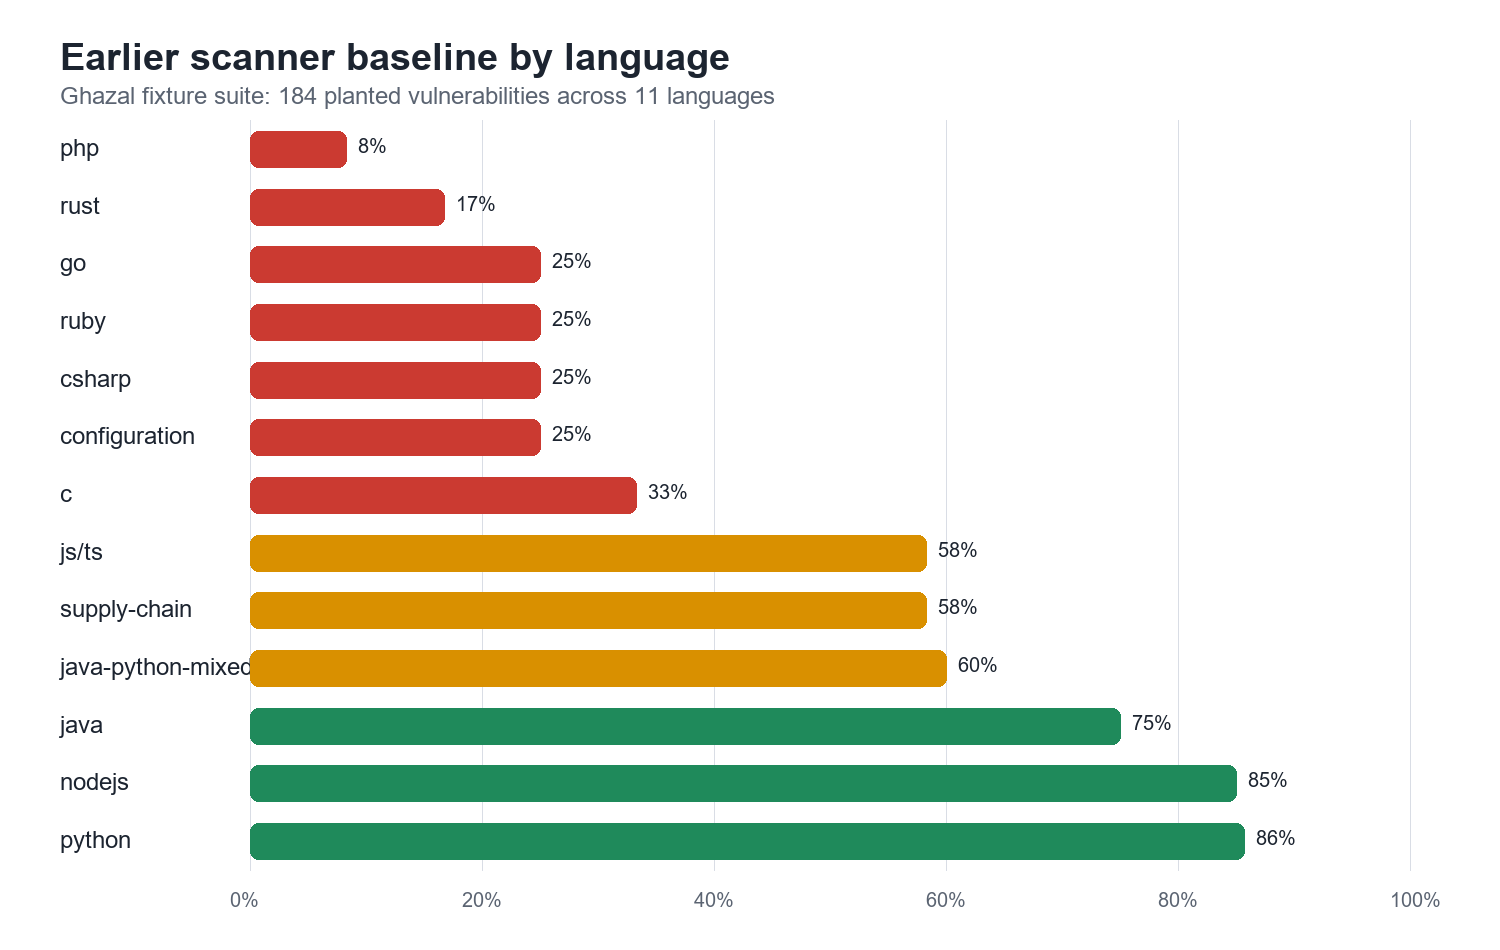
\includegraphics[width=\linewidth]{figures/language_baseline.png}
  \caption{Earlier scanner-only baseline by language. HermSec performed best on Python, Node.js, and Java.}
  \Description{A horizontal bar chart showing scanner-only detection rates by language. Python and Node.js are high. PHP, Rust, Go, Ruby, C sharp, and configuration are lower.}
  \label{fig:language-baseline}
\end{figure}

\subsection{Final Mode Comparison}
Table~\ref{tab:mode-summary} shows the final results. Deep assisted scan found the most real issues, but it also reported many extra findings. Single agent inspection reported very few findings, so it had better precision, but it missed many bugs. MoA inspection gave a better balance than one agent. Scanner + MoA had the best F1 score in this test. It found fewer true positives than deep assisted scan, but it reduced the scanner false positives sharply.

\begin{table*}
  \caption{Aggregate results across four controlled fixtures.}
  \label{tab:mode-summary}
  \centering
  \small
  \begin{tabular}{lrrrrrrr}
    \toprule
    Mode & Runs & TP & FP & FN & Precision & Recall & F1 \\
    \midrule
    Deep assisted & 4 & 8 & 81 & 4 & 0.0899 & 0.6667 & 0.1584 \\
    Single agent & 4 & 2 & 1 & 10 & 0.6667 & 0.1667 & 0.2667 \\
    MoA assisted & 4 & 5 & 4 & 7 & 0.5556 & 0.4167 & 0.4762 \\
    Scanner + MoA & 4 & 7 & 9 & 5 & 0.4375 & 0.5833 & 0.5000 \\
    \bottomrule
  \end{tabular}
\end{table*}

\begin{figure*}
  \centering
  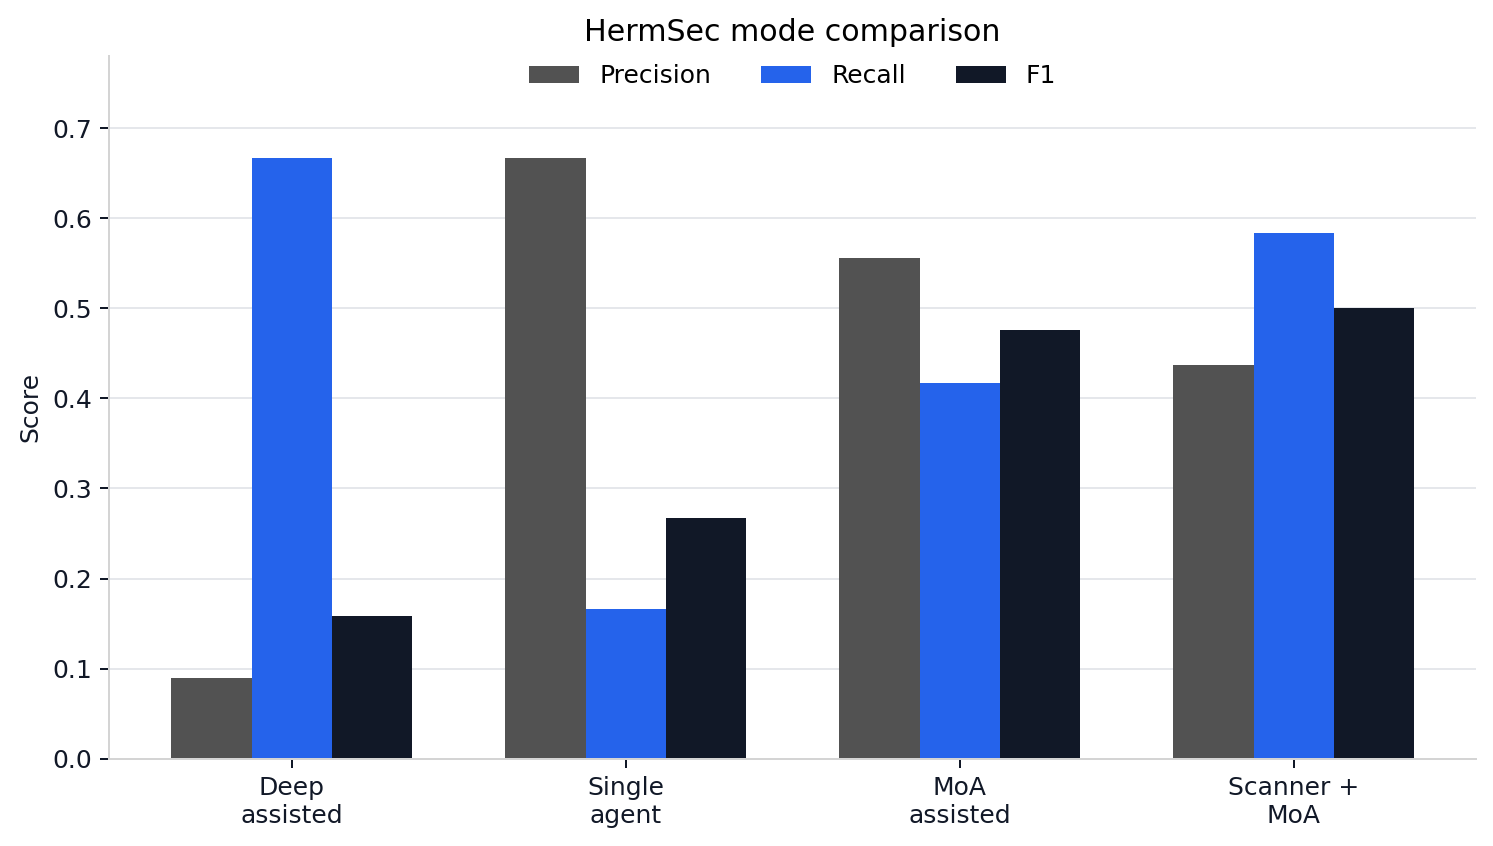
\includegraphics[width=.48\textwidth]{figures/mode_metrics.png}\hfill
  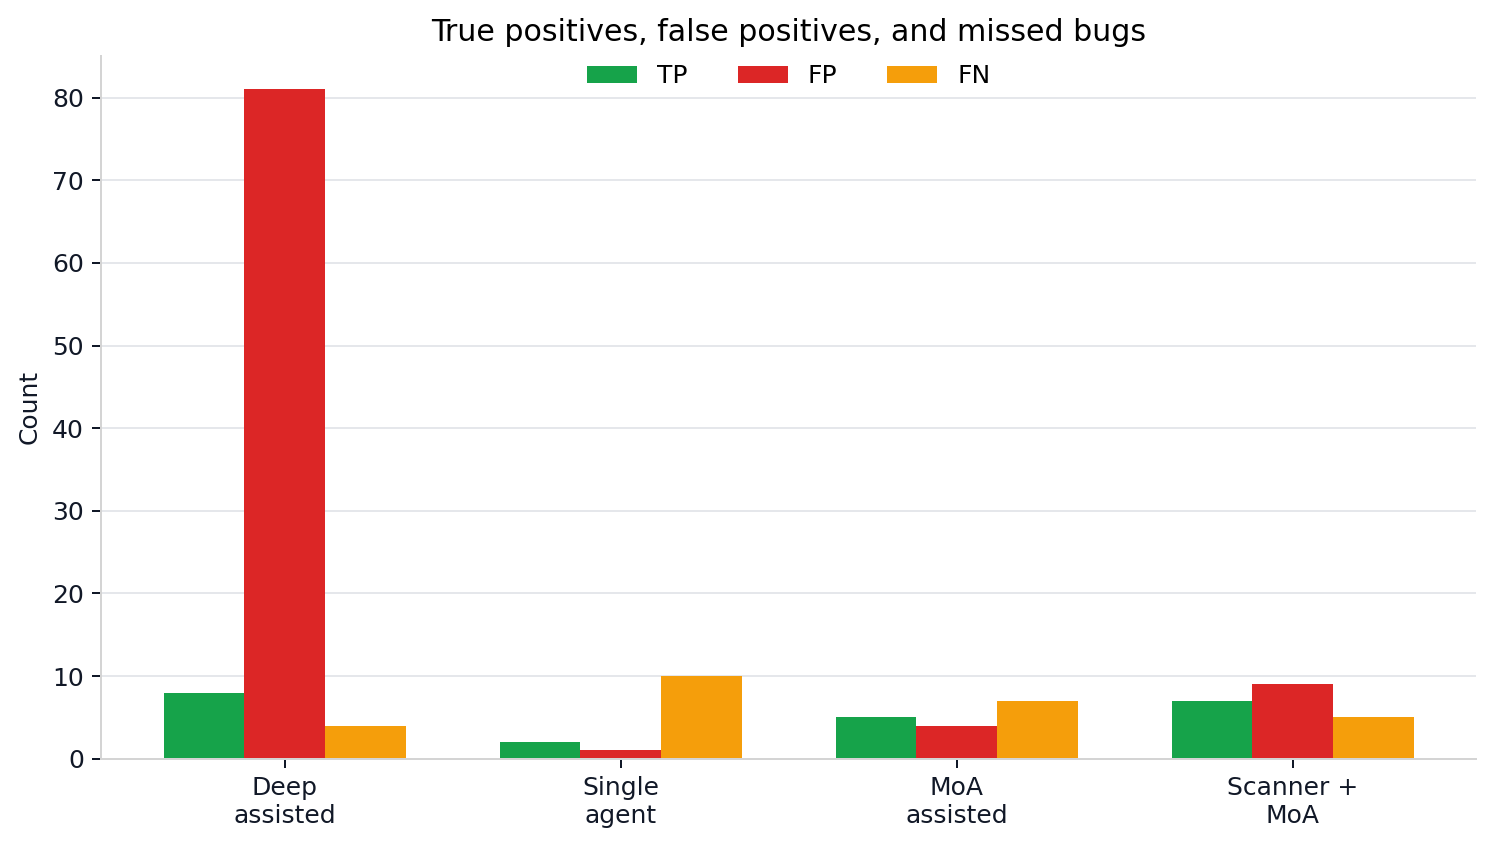
\includegraphics[width=.48\textwidth]{figures/mode_counts.png}
  \caption{Final mode comparison. Left: precision, recall, and F1. Right: true positives, false positives, and false negatives.}
  \Description{Two bar charts. The left chart compares precision, recall, and F1 for deep assisted, single agent, MoA assisted, and Scanner plus MoA modes. The right chart compares true positives, false positives, and false negatives for the same modes.}
  \label{fig:mode-comparison}
\end{figure*}

\subsection{Per-Fixture Results}
Table~\ref{tab:fixture-results} gives the detailed results. Single agent and MoA both returned zero findings on the clean projects. This is good because the clean projects should not produce findings.

On the vulnerable projects, MoA found three Node.js issues and two Python issues. Single agent only found one issue in each vulnerable project. Deep assisted found more planted issues, especially in the Python project, but it also reported many findings that were outside the answer key. Scanner + MoA found four Node.js issues and three Python issues. It still had some false positives, but it gave the best total F1 score.

\begin{table*}
  \caption{Per-fixture results from the final comparison.}
  \label{tab:fixture-results}
  \centering
  \small
  \begin{tabular}{llrrrrrr}
    \toprule
    Fixture & Mode & Findings & Expected & TP & FP & FN & F1 \\
    \midrule
    Node vulnerable & Deep assisted & 25 & 6 & 3 & 22 & 3 & 0.1935 \\
    Node clean & Deep assisted & 6 & 0 & 0 & 6 & 0 & 0.0000 \\
    Python vulnerable & Deep assisted & 57 & 6 & 5 & 52 & 1 & 0.1587 \\
    Python clean & Deep assisted & 1 & 0 & 0 & 1 & 0 & 0.0000 \\
    Node vulnerable & Single agent & 2 & 6 & 1 & 1 & 5 & 0.2500 \\
    Node clean & Single agent & 0 & 0 & 0 & 0 & 0 & 1.0000 \\
    Python vulnerable & Single agent & 1 & 6 & 1 & 0 & 5 & 0.2858 \\
    Python clean & Single agent & 0 & 0 & 0 & 0 & 0 & 1.0000 \\
    Node vulnerable & MoA assisted & 6 & 6 & 3 & 3 & 3 & 0.5000 \\
    Node clean & MoA assisted & 0 & 0 & 0 & 0 & 0 & 1.0000 \\
    Python vulnerable & MoA assisted & 3 & 6 & 2 & 1 & 4 & 0.4444 \\
    Python clean & MoA assisted & 0 & 0 & 0 & 0 & 0 & 1.0000 \\
    Node vulnerable & Scanner + MoA & 10 & 6 & 4 & 6 & 2 & 0.5000 \\
    Node clean & Scanner + MoA & 1 & 0 & 0 & 1 & 0 & 0.0000 \\
    Python vulnerable & Scanner + MoA & 4 & 6 & 3 & 1 & 3 & 0.6000 \\
    Python clean & Scanner + MoA & 1 & 0 & 0 & 1 & 0 & 0.0000 \\
    \bottomrule
  \end{tabular}
\end{table*}

\section{Discussion}
\subsection{Answer to RQ1}
Scanner + MoA had the best F1 score in this test. Deep assisted scan had the best recall, but it had too many false positives. Single agent inspection was cleaner, but it missed too many planted bugs. MoA was a strong middle point, but the hybrid mode performed slightly better overall.

\subsection{Answer to RQ2}
MoA did reduce noise compared with the scanner-based mode. It also found more real bugs than the single agent. This shows that the judge and aggregator can help. However, MoA still missed 7 of 12 planted vulnerabilities. This means it is useful, but it is not enough by itself.

\subsection{Answer to RQ3}
Scanner + MoA improved the balance in this small test. It reached F1 0.500, which was higher than MoA at 0.476. It also found 7 true positives, compared with 5 for MoA and 2 for the single agent. However, it still produced 9 false positives, so the judge and aggregator need more tuning.

\subsection{Answer to RQ4}
The next step is better coverage. HermSec still needs stronger language-specific rules and scanners for PHP, Go, Ruby, Rust, C\#, C/C++, and configuration files. The agent modes should also be tested on larger public benchmarks. Deep assisted scan should be tested again after the model fallback issue is fixed. Scanner + MoA should also be tested with different candidate limits because too many scanner candidates can make the final aggregator fail or become noisy.

\section{Threats to Validity}
This study is small. The final comparison used only four fixtures and 12 planted vulnerabilities. The results show a useful direction, but they do not prove that the same result will happen on all projects.

The bugs were also synthetic. Real projects can have more complex code and more complex data flow. The scoring method can also count a useful scanner finding as a false positive if it is not in the answer key. This affected the deep assisted results. Finally, model behavior can change because of provider errors, prompt changes, timeout settings, and model updates.

\section{Future Work}
Future work should test HermSec on larger benchmarks. Good next benchmarks are OWASP BenchmarkJava, OpenSSF CVE Benchmark, CASTLE, and selected Juliet test cases. HermSec should also improve Java taint tracking, scanner installation, benchmark exports, and cost tracking for model runs. Another useful test would compare different MoA panel sizes, different judge settings, and different Scanner + MoA candidate limits.

\section{Conclusion}
This paper presented HermSec as a user-friendly repository security scanner and compared four HermSec review modes. Deep assisted scan found the most planted bugs, but it had many false positives. Single agent inspection was clean, but it missed many bugs. MoA inspection gave a better balance than one agent. Scanner + MoA had the best F1 score in this small test.

The main conclusion is simple. Scanners are still needed for broad coverage. Agent modes are useful for cleaner review and explanation. The hybrid Scanner + MoA direction looks promising because it combines both ideas. It still needs larger testing before strong claims can be made.

\begin{acks}
This work was developed for Security Insider Lab II. I thank my colleague Ghazal for preparing the broader fixture tests and benchmark notes used for the scanner-only baseline.
\end{acks}

\bibliographystyle{ACM-Reference-Format}
\bibliography{hermsec_moa_refs}

\end{document}
